\chapter{Basics}\label{ch:basics}

The chapter provides the groundwork necessary for the comparative analysis of automatic 3D model generation techniques by introducing the key technologies that drive these methods. It is essential to have a common understanding of the generative machine learning algorithms and 3D data representations that form the basis of this field.

The section starts with Variational Autoencoders (VAEs) \citep{kingmaVAE,rezendeVAE}, which serve as probabilistic frameworks for learning complex data representations. Generative Adversarial Networks (GANs) \citep{goodfellowGAN} are then discussed, highlighting their unique training dynamics that include both generator and discriminator components. The section further explores the domain of Diffusion Models, particularly Denoising Diffusion Probabilistic Models (DDPMs) \citep{hoDDPMs,sohlDDPM}, while also briefly covering Stochastic Gradient Methods (SGMs) \citep{song2019SGM} and Stochastic Differential Equations (SDEs) \citep{song2020score,song2021maximum}. These mentioned models, as captured by the ``generative learning trilemma'' \citep{xiao2022tackling}, highlight the balance and compromises inherent in their design and application.

\begin{figure}[ht]
    \centering
      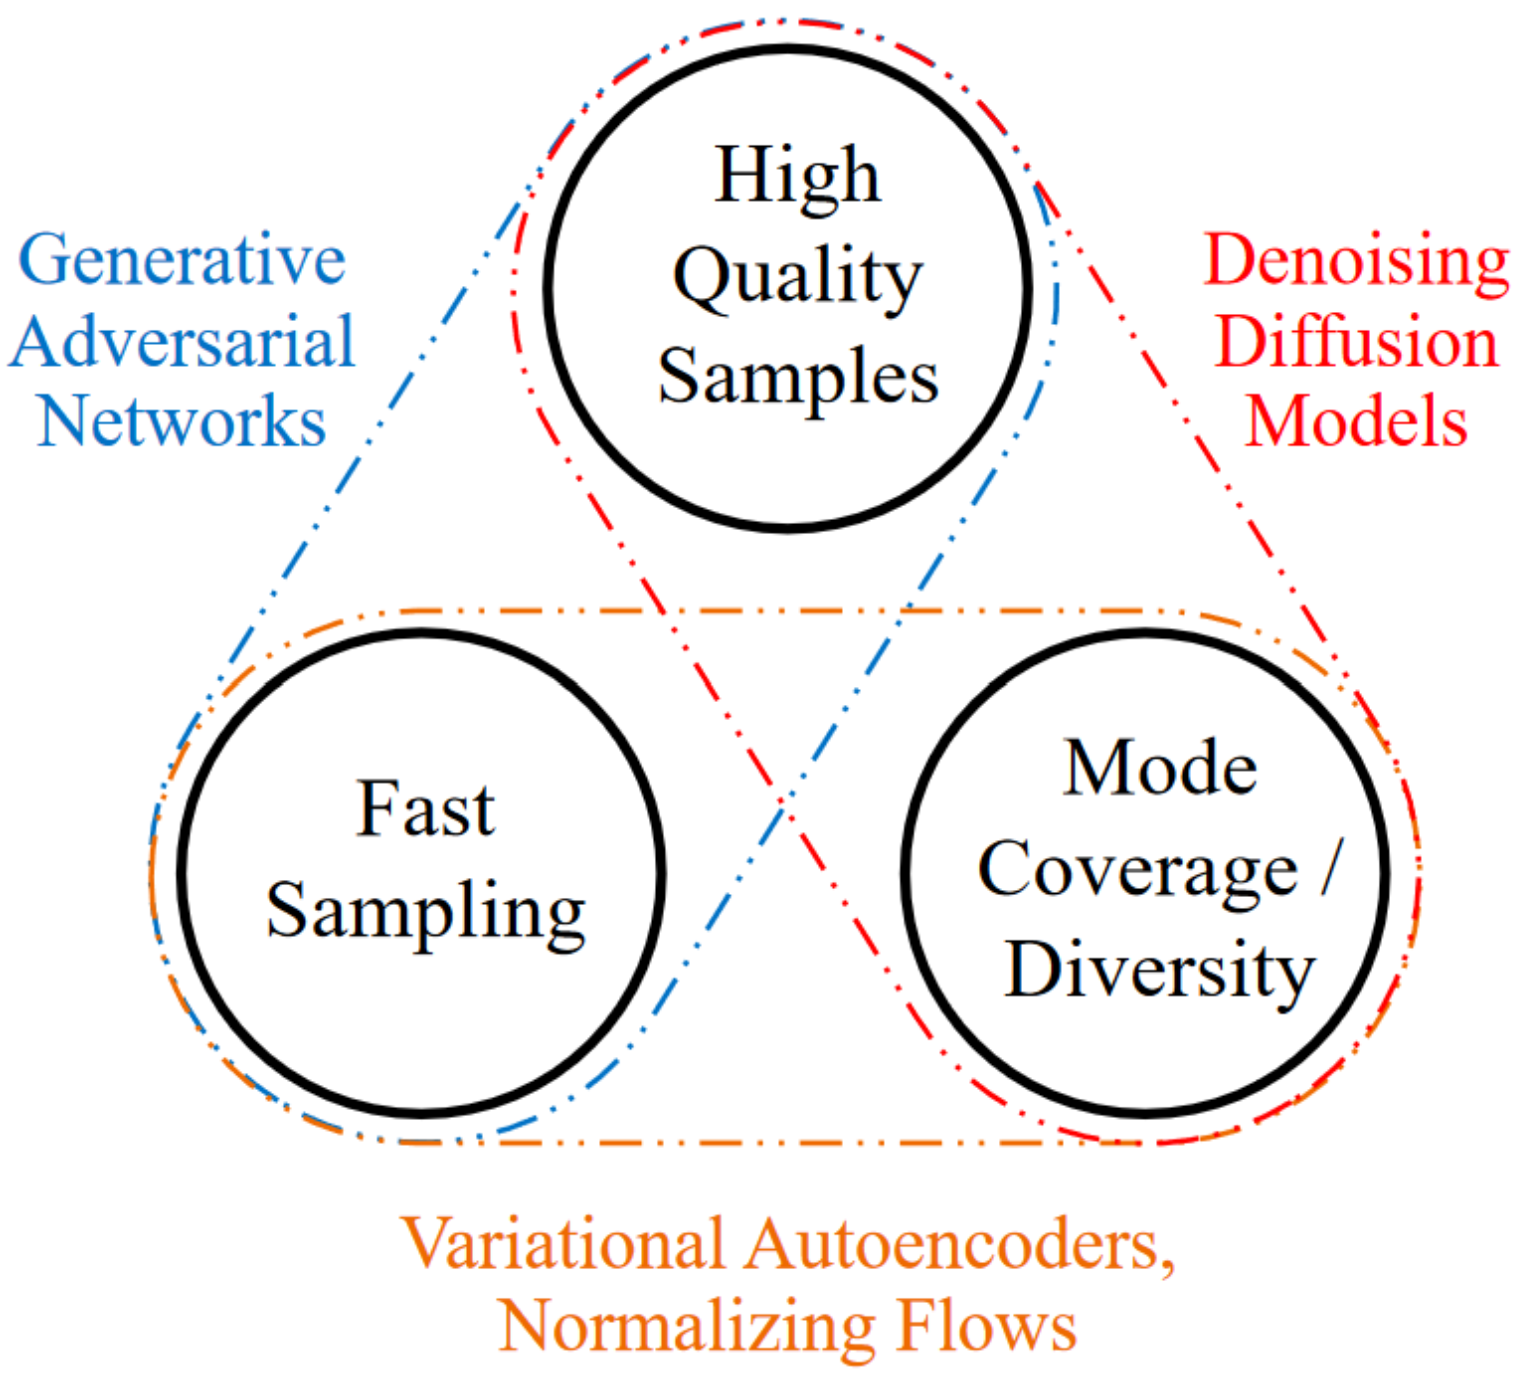
\includegraphics[width=.4\columnwidth]{figures/BasicTrilemma.png}
      \caption{A short characterization of the most important features and drawbacks of the generative models discussed in this section.~\citep{xiao2022tackling}}\label{fig:generativeTrilemma}
\end{figure}

The chapter also examines Contrastive Language-Image Pre-training (CLIP) \citep{radfordCLIP}, showcasing its ability to bridge natural language and visual data, thereby facilitating text-guided 3D model generation. Lastly, various forms of representation of 3D data are examined, including Meshes, Point-Clouds, and Voxels, constituting the foundational structure of 3D objects in computational environments. Proficiency in these representations is required for comprehending the 3D model generation.

//TODO check Final Diffusion Model

\section{Variational Autoencoders - VAEs}
\label{VAEs}

Based on the seminal work by \citeauthor{diggleImplicitPrescribed}, generative models can be classified into two broad categories. Prescribed models employ a well-defined, often parametric, mathematical expression for the probability density function (pdf), which enables easier analytical interpretation of the distributions. In contrast, implicit models synthesize new data samples without relying on an explicit pdf, approximating the underlying data distribution on which they were trained \citep{diggleImplicitPrescribed}. Variational Autoencoders (VAEs), which inherit the foundational architecture of autoencoders, belong to the prescribed models category as they require an explicit formulation of the probability density function (pdf) to function effectively. This feature makes VAEs suitable for tasks that require not only the generation but also the understanding of complex data distributions. \citep{kingmaVAE,rezendeVAE,GoodfellowDeepLearning}. Generative Adversarial Networks (GANs) \citep{goodfellowGAN}, discussed later, are a prime example ofthe latter category.

VAEs are essentially based on the architecture of autoencoders, which consist of an encoder and a decoder. The encoder aims to transform the input data into a low-dimensional latent space representation, commonly referred to as a "code" or "bottleneck" \citep{hintonCode, GoodfellowDeepLearning}. This code captures the most relevant features of the input while reducing its dimensionality. Then, the decoder attempts to reconstruct the original input from the obtained latent vector using a loss function. As explained by Goodfellow et al, an autoencoder that only succeeds in copying the exact representation of the input data does not itself prove useful. The essence of autoencoders lies in their ability to copy approximately rather than perfectly, which forces the model to prioritize which aspects of the input to copy \citep{GoodfellowDeepLearning}. This strategic approach often directs autoencoders to "learns useful properties of the data" \citep{GoodfellowDeepLearning}. To summarize, he main goal of an autoencoder is not the reconstruction itself, but the extraction of a meaningful latent vector that serves as a simplified representation of the input data.

The ability to reduce dimensionality has practical implications for improving the efficiency of classification tasks by reducing computational and memory overhead \citep{GoodfellowDeepLearning}. When paired with information retrieval, this dimensionality reduction makes searching in certain low-dimensional spaces particularly efficient \citep{GoodfellowDeepLearning}. Despite these advantages, traditional autoencoders are not designed to generate new data; their main function is to copy and reconstruct the given input \citep{GoodfellowDeepLearning}.

\begin{figure}[ht]
    \centering
      \hspace{.8cm}
      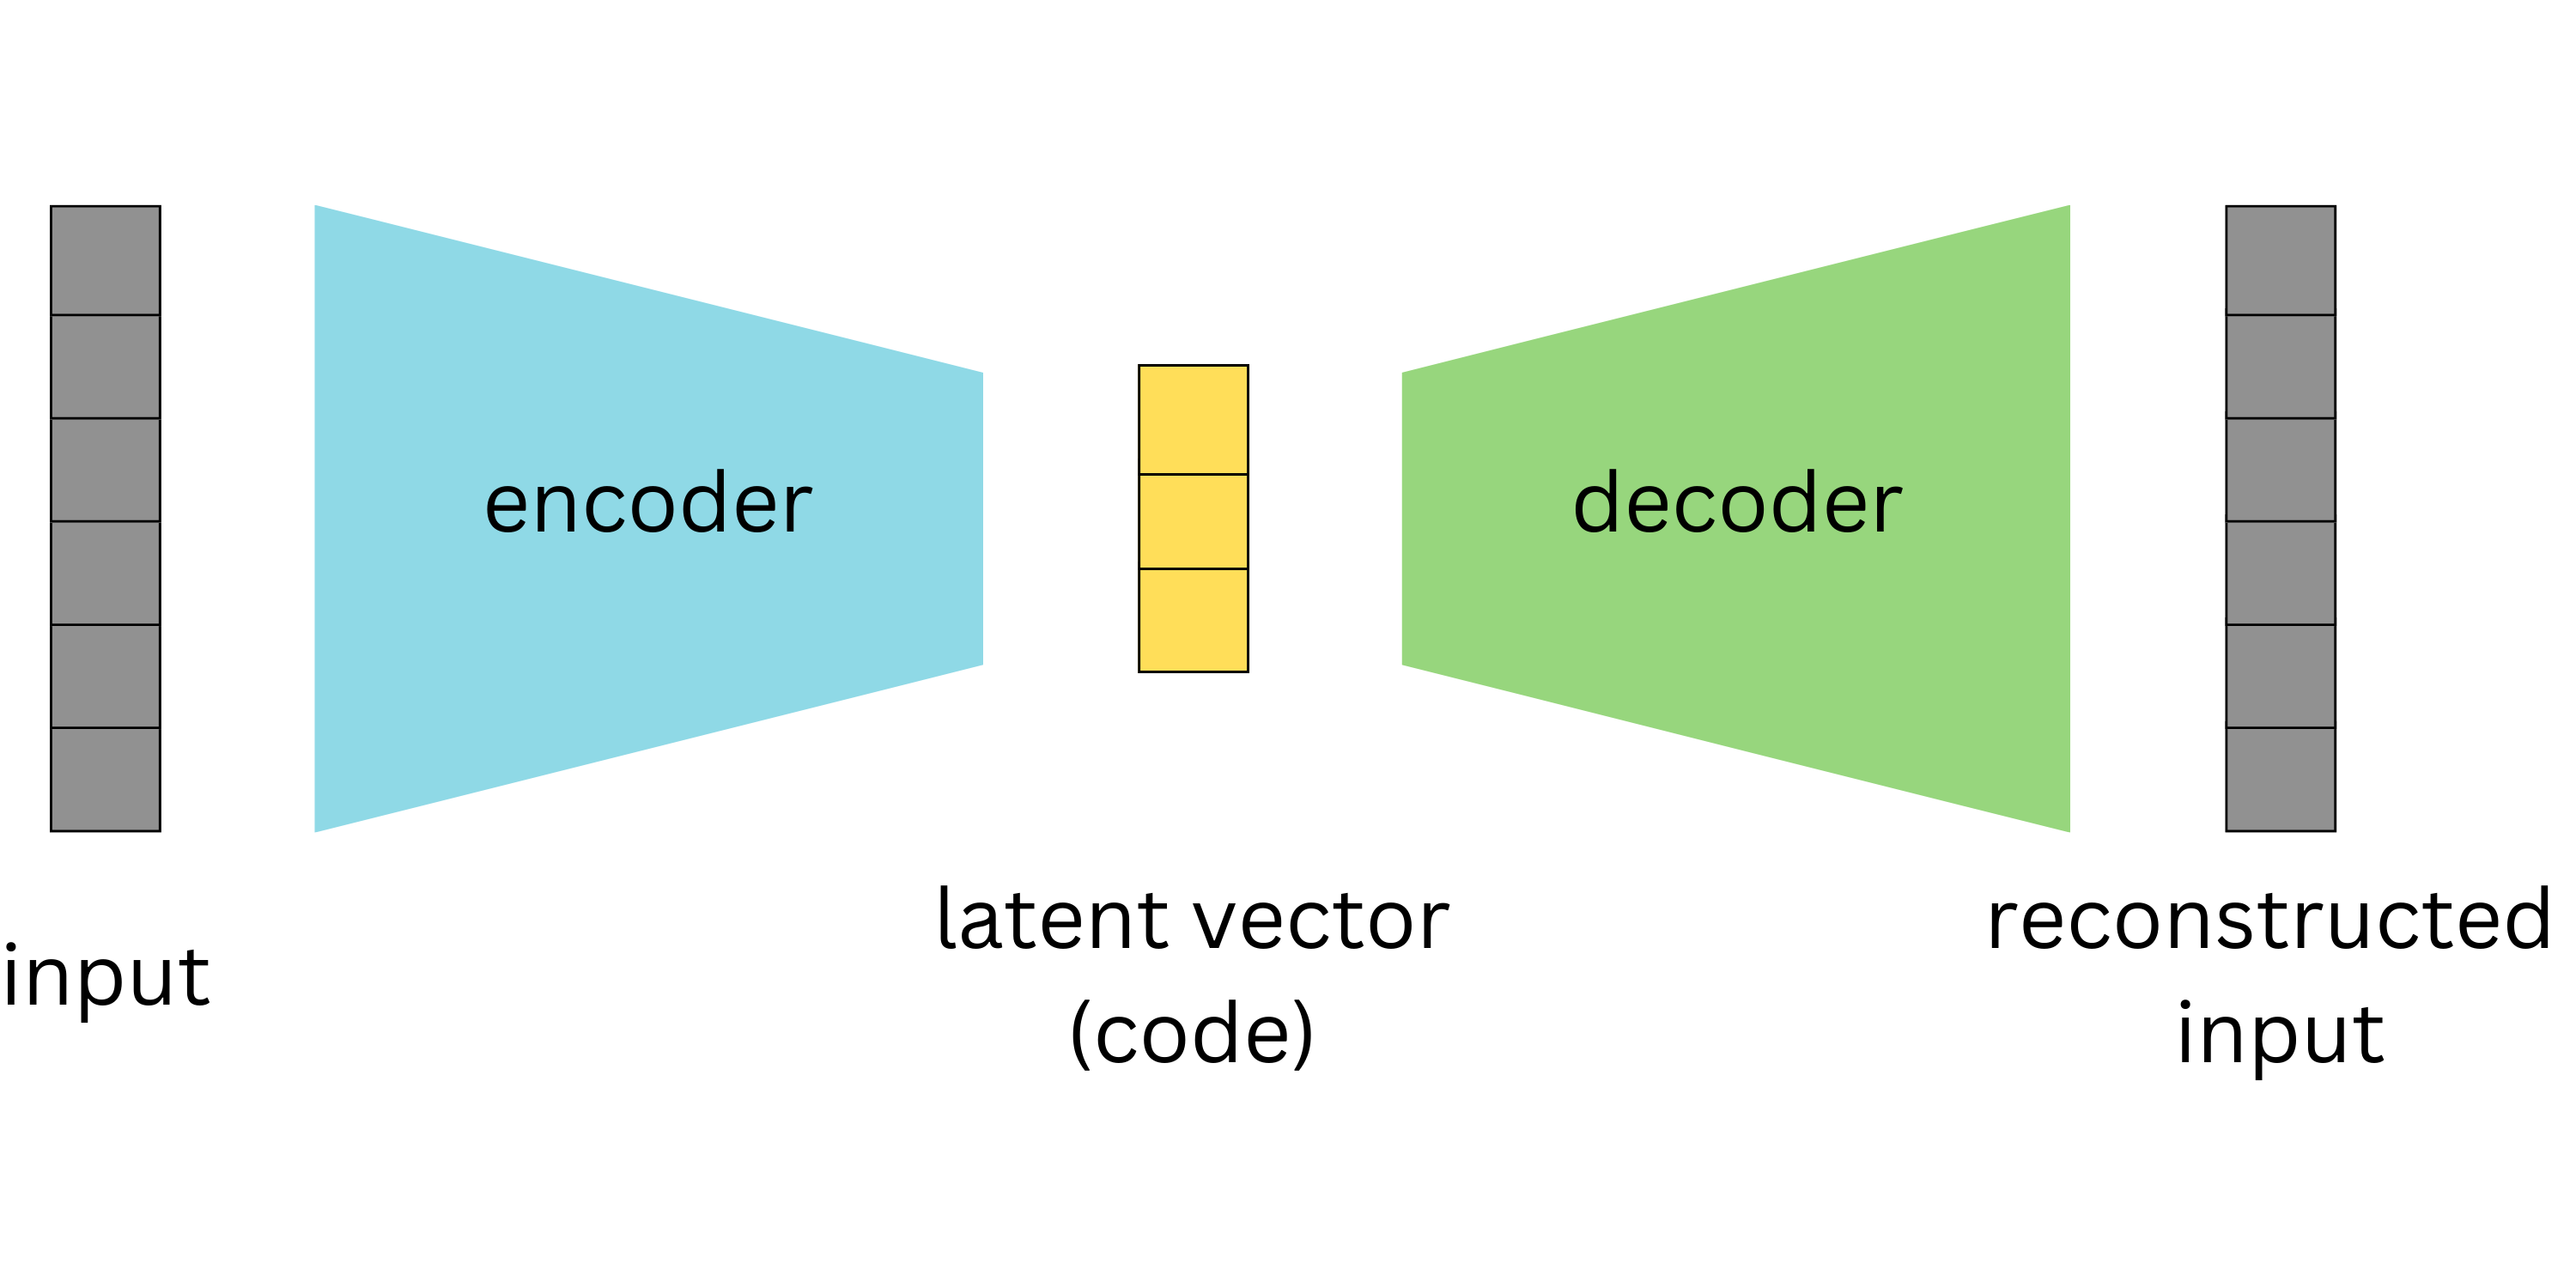
\includegraphics[width=.7\columnwidth]{figures/Autoencoder.png}
      \caption{Autoencoder: The encoder reduces the input dimension to a latent vector that captures the most important features. The decoder then uses this vector to reconstruct the input, with training aimed at minimizing reconstruction loss.}
      \label{fig:figureAE}
    \end{figure}


In variational autoencoders (VAEs), the encoder compresses the input into a space of latent variables and forms a probability distribution over these latent variables called \( q(z|x) \). This distribution helps with robustness against overfitting and enables the model to synthesize new analog data points. During the training phase, VAEs recognize specific regions in the latent variable space, similar to "pools," for different categories of data, allowing for a structured approach to data representation. Unlike standard autoencoders, where it is unclear where a useful latent vector can be sampled for the decoder, VAEs overcome this problem by restricting the latent space to known regions from which vectors can be safely sampled, as cited in \citep{doerschVAE}.

The procedure begins by selecting a sample \( z \) from a code distribution defined by the model, denoted \( p_{model}(z) \). This sample \( z \) is then passed through a differentiable generator network \( g(z) \). A sample \( x \) is then drawn from the distribution \( p_{model}(x; g(z)) \), where its properties are shaped by the processed \( z \) \citep{GoodfellowDeepLearning}. During the training phase, an approximate inference network, also called an encoder \( q(z|x) \), is used to infer \( z \) from \( x \), while \( p_{model}(x|z) \) works as a decoder network to reconstruct \( x \) from \( z \) \citep{GoodfellowDeepLearning}. The main training objective is embodied in the formula:
        
\begin{align}
  L(q) &= \mathbb{E}_{z \sim q(z|x)} \log p_{model}(z, x) + H(q(z|x)) \\
  &= \mathbb{E}_{z \sim q(z|x)} \log p_{model}(x|z) - D_{KL}(q(z|x) || p_{model}(z)) \\
  &\leq \log p_{model}(x)
\end{align}
        
Here, \( L(q) \) acts as a scorecard to evaluate the performance of UAE. The first term \( \log p_{\text{model}}(x|z) \) evaluates how well the UAE can fill in the details to recover the original input, while the second term \( D_{\text{KL}}(q(z|x) || p_{\text{model}}(z)) \) evaluates the complexity of the VAE representation compared to the original term, aiming for simplicity, as mentioned in \citep{GoodfellowDeepLearning}. 
        
The decoder in VAEs either reconstructs the original input or synthesizes new outputs from sampled latent variables. This process is optimized by a loss function that includes both the reconstruction loss and a regularization term based on the Kullback-Leibler (KL) divergence \( D_{\text{KL}} \). This divergence measures the discrepancies between the estimated and true data distributions \citep{kingmaVAE} and improves the model's ability to effectively generalize to unseen data.
        
Through this mechanism, VAEs continuously refine their representation and reconstruction process, improving the generation of new data points that resemble the original training data while maintaining a simplified and structured latent space.

\begin{figure}[ht]
    \centering
      \hspace{.8cm}
      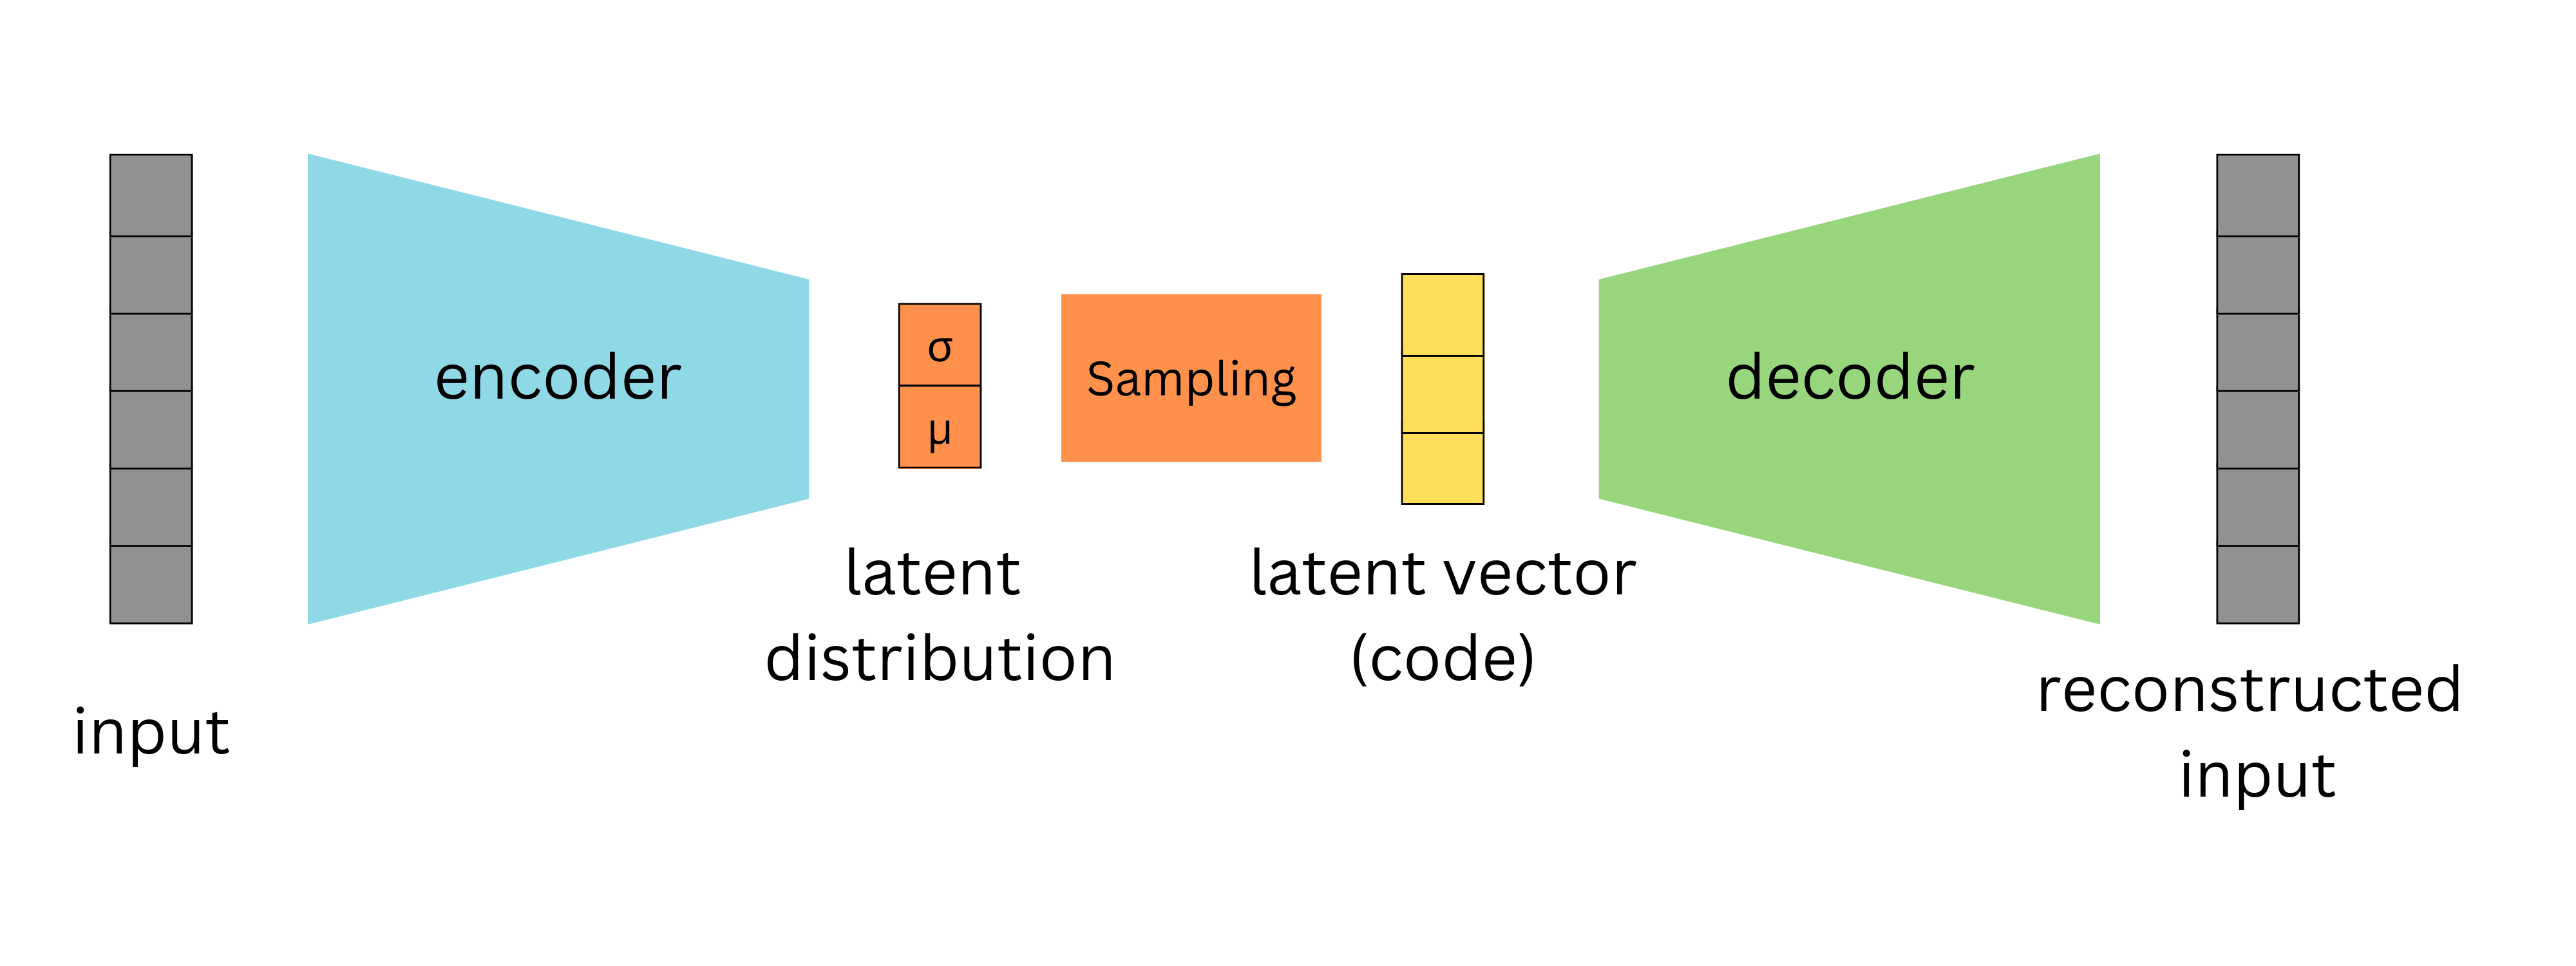
\includegraphics[width=.9\columnwidth]{figures/VAE.png}
      \caption{Functionality of a Variational Autoencoder, demonstrating incorporation of the latent distribution - the mean and standard deviation - for enhancing generative capabilities.}
      \label{fig:figureVAE}
\end{figure}

Despite their capabilities, VAEs exhibit some limitations. According to \citeauthor{GoodfellowDeepLearning}, the generated samples can often be blurry. The reason for this is not fully 
understood, but the blurriness observed may be due to their optimization process, which minimizes Kullback-Leibler divergence. This could lead the model to assign high probabilities to "points that occur in the training set, but may also assign high probability to other points [...] which may include blurry images" \citep{GoodfellowDeepLearning}. The Gaussian distribution often used in VAEs for the generative model may also contribute to this effect, as it can ignore minor features in the input data \citep{GoodfellowDeepLearning}. Another issue is that VAEs typically utilize only a small portion of the latent space, which might further compromise the quality of generated images \citep{GoodfellowDeepLearning}. The performance of the model is also sensitive to the choice of priors for the latent space, making hyperparameter tuning an essential aspect of working with VAEs \citep{kingmaVAE, higginsVAE}. 


\section{Generative Adversarial Networks~--~GANs}\label{GAN}

``When a deep neural network is used to generate data, the corresponding density function may be computationally intractable'' \citep{goodfellowGAN}. Unlike traditional generative models, implicit generative models do not require the explicit design of a density function to describe the patterns in the data. Instead, they use a sample generation process that produces new samples resembling the existing ones \citep{goodfellowGAN}. Before Generative Adversarial Networks were introduced, the leading implicit generative model was the generative stochastic network, ``which is capable of approximately generating samples via an incremental process based on Markov chains'' \citep{goodfellowGAN}. Markov chains are a way of describing a sequence of events or states, where probability of transition to the succeeding state is solely dependent on current states. This approach, however, can be time-intensive and may not always yield accurate results. GANs, on the other hand, directly generate high-quality samples in a single step, bypassing the gradual and often inefficient process of incremental generation.

The unique adversarial nature of GANs arises from the game-like competition between two neural networks: the generator and the discriminator. The generator is responsible for creating fake inputs or samples, which are then passed to the discriminator. The discriminator's role is to differentiate between real samples from the domain set and the fake samples generated by the generator.

\begin{figure}[ht]
\centering
  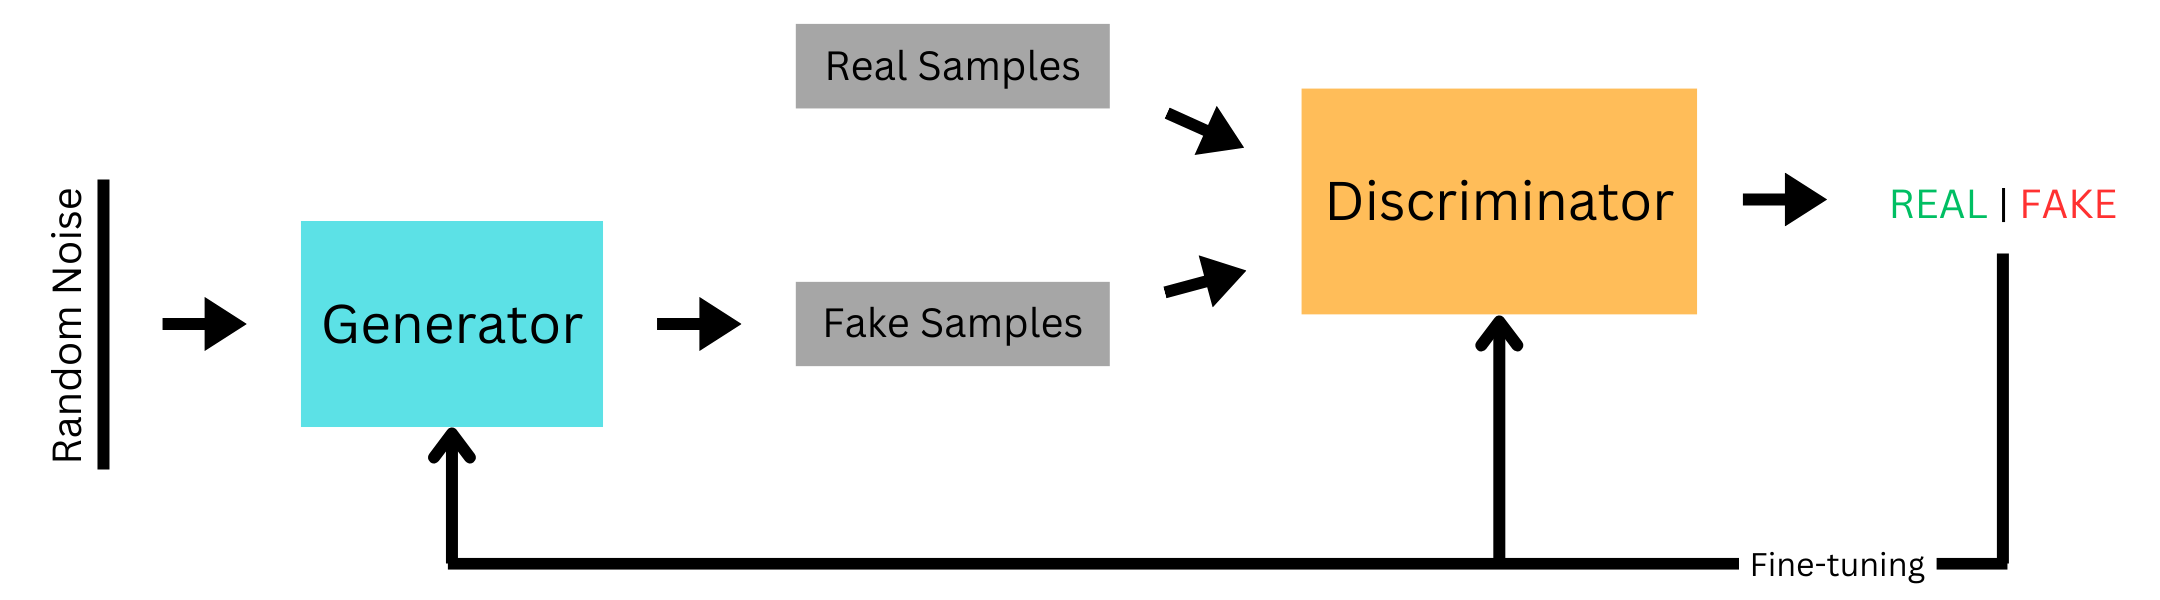
\includegraphics[width=1\columnwidth]{figures/Generator.png}
  \caption{Schematic representation of Generative Adversarial Networks showcasing the interaction between the generator and discriminator networks in generating new data.}\label{fig:figureGAN}
\end{figure}

In the initial training phase, the discriminator is trained on a dataset of real, unlabeled data, learning to identify the characteristics of authentic samples. As the discriminator becomes adept at recognizing all details, the generator starts creating counterfeits, using random input vectors to produce imitations. The discriminator then evaluates these fakes and provides feedback. This feedback loop, involving sample creation and model adjustments, gradually refines the generator's output. Eventually, the generator becomes so proficient that its fakes are indistinguishable from real data, achieving what is known as a zero-sum game, where one network's gain is the other's loss \citep{goodfellowGAN}.

However, the utility of GANs extends far beyond just image generation. Their applications encompass a wide range of fields, demonstrating their versatility and significant impact. These applications include video frame prediction, which is essential in multimedia applications; image enhancement, crucial in improving the quality and clarity of visual data; and encryption, where GANs contribute to the development of advanced security protocols \citep{goodfellowGAN}. One of the most notable features of GANs is their ability to learn in an unsupervised manner, particularly through the generator network. Unlike traditional models that require a supervised learning set with labeled data, GANs can generate new data after training the discriminator with real examples. This capability allows GANs to produce realistic and varied outputs without direct exposure to or reliance on a large labeled dataset \citep{GoodfellowDeepLearning},

% Additionally, GANs play a pivotal role in 3D object generation, the medical field,computer vision as well as traffic control systems, aiding in the development of smarter and more efficient transportation management \citep{AGGARWAL2021100004}.

Nevertheless, GANs pose a substantial challenge in their training process as they are hard to train \citep{goodfellowGAN}. In addition, \citeauthor{brophyGAN} highlight three important problems commonly associated with GANs, among others. These issues, namely non-convergence, diminishing or vanishing gradients, and mode collapse, contribute to the inherent instability experienced during GAN training. Non-convergence refers to the failure of a GAN model to stabilize and reach a state of equilibrium. Instead, it continuously oscillates and fails to converge to a satisfactory solution. As a result, the model does not learn the underlying patterns of the data and can even diverge, leading to poor performance \citep{brophyGAN}. Diminishing or vanishing gradients occur when the gradients used to update the generator become extremely small or even vanish altogether. This phenomenon is often caused by an overly successful discriminator that becomes too adept at distinguishing real and fake samples. As a result, the generator struggles to learn from the feedback provided by the discriminator, impeding its ability to generate high-quality samples \citep{brophyGAN}. Mode collapse happens when the generator collapses, meaning it focuses on producing only a limited set of samples or outputs, typically lacking diversity and variety \citep{salimansNIPS}. In such cases, the generator fails to capture the full range of patterns and characteristics present in the training data, resulting in uniform and repetitive samples that do not adequately represent the true distribution \citep{brophyGAN}.
\section{Diffusion models}
\label{diffusion Models}

The limitations of VAEs and GANs, which were just stated above, have led to the emergence of diffusion models, a method that offer distinct advantages over traditional generative models. Diffusion models operate by progressively perturbing data with noise and then learning to reverse this process to generate new samples. 

~\cite{yangdiffusionSummary} distingueshe between three main approaches that dominate the study of diffusion models, which are going to be discussed shortly: Denoising Diffusion Probabilistic Models (DDPMs) \citep{hoDDPMs,sohlDDPM}, Score-based Generative Models (SGMs) \citep{song2019SGM}, and Stochastic Differential Equations (Score SDEs) \citep{song2020score, song2021maximum}.

\subsection{Denoising Diffusion Probabilistic Models}
DDPMs employ two Markov chains, a forward chain and a reverse chain, also known as the forward and reverse diffusion processes, seen in Figure~\ref{fig:figureForwardProcess} and Figure~\ref{fig:figureReverseProcess} \citep{sohlDDPM}. 

The forward diffusion process is comparable to latent variable models, sharing some similarities with Variational Autoencoders (VAEs), as focus is lying on a latent feature space of the initial data distribution. They differ in the fact that the forward process in DDPMs "is fixed to a Markov chain that gradually [over a span of T steps] adds Gaussian noise to the data according to a variance schedule \(\beta_1, ..., \beta_T \)" \cite{hoDDPMs}. This iterative process continues to add noise "until all structures are lost" \citep{yangdiffusionSummary} resulting in an image of pure noise. The introduction of noise aims to gradually steer the data distribution towards a more manageable prior distribution \citep{yangdiffusionSummary, pooleDreamfusion}. Mathematically, the forward process can be described in two equations:

\[
q(x_t | x_{t-1}) = \mathcal{N}(x_t; \sqrt{1 - \beta_t}x_{t-1}, \beta_t I) \quad \text{where} \quad \sqrt{1 - \beta_t}x_{t-1} = \mu_t \quad \text{and} \quad \beta_t I = \Sigma_t
\] 

\citep{martinez2023understanding}. This describes the process of adding noise to transform a data point \( x_{t-1} \) into a new data point \( x_t \). This transformation is probabilistic and follows a Gaussian distribution \citep{sohlDDPM, hoDDPMs}. The mean value of this distribution is slightly adjusted compared to the previous data point by the factor \( \sqrt{1 - \beta_t} \), which essentially corresponds to the data point \( x_{t-1} \) with a certain noise reduction. The parameter \( \beta_t \) controls the amount of noise added, where a larger \( \beta_t \) means more noise \citep{kingma2023variationalDM}. The covariance matrix, denoted \( \beta_t I \), implies that each element of the data is independently modified with the same amount of noise, since \(I\) represents an identity matrix where all outer diagonal elements are zero \citep{croitoru2023diffusion}.

\[q(x_{1:T} | x_0) = \prod_{t=1}^T q(x_t | x_{t-1}) \] 

\citep{martinez2023understanding}. In the second equation, the focus is on the entire sequence of data points from the original \( x_0 \) to \( x_T \), including all intermediate points \citep{martinez2023understanding}. This expresses the idea that to understand the probability of the entire noisy trajectory, one can calculate the probability of each step from \( x_{t-1} \) to \( x_t \) and then multiply these probabilities together. This is due to the Markov property, which states that each step is only dependent on the immediately preceding step \citep{martinez2023understanding}. This enables a comprehensive view of the transition probabilities over the entire process of noise induction, step by step.

\begin{figure}[ht]
\centering
  \includegraphics[width=1\columnwidth]{figures/manta_DDMP3.png}
  \caption{Forward process adding noise to an image}
  \label{fig:figureForwardProcess}
\end{figure}

The reverse chain is trained to approximate the inverse of the forward process using a deep neural network parameterized with~\(\Theta\), effectively removing the noise added by the forward chain \citep{sohlDDPM, yangdiffusionSummary}. The function \( p_\theta(x_{t-1} | x_t) \) is a probability distribution that estimates how to reverse the diffusion process. Given a data point \( x_t \), it attempts to predict the previous data point \( x_{t-1} \) before noise was added. It is modeled as a normal distribution with a mean \( \mu_\theta(x_t, t) \) and covariance \( \Sigma_\theta(x_t, t) \), both of which are functions parameterized by \( \theta \) \citep{yangdiffusionSummary}.

\[
  p_\theta(x_{t-1} | x_t) = \mathcal{N}(x_{t-1}; \mu_\theta(x_t, t), \Sigma_\theta(x_t, t))
\] 

\[p_\theta(x_{0:T}) = p_\theta(x_{T}) \prod_{t=1}^T p_\theta(x_{t-1} | x_t) \]

\citep{martinez2023understanding}. The latter function \( p_\theta(x_{0:T}) \) represents the probability of the entire sequence of data points from \( x_0 \) through \( x_T \) under the reverse process modeled by the neural network. It starts with an estimate of the final data point \( p_\theta(x_{T}) \) and works backwards through the sequence, multiplying the conditional probabilities \( p_\theta(x_{t-1} | x_t) \) for each step \citep{hoDDPMs,martinez2023understanding}. This function essentially provides a framework for reconstructing the original data from the noisy data by successively removing noise at each step, based on the learned parameters \( \theta \) \citep{yangdiffusionSummary}.


\begin{figure}[ht]
  \centering
    \includegraphics[width=1\columnwidth]{figures/manta_DDMP3.png}
    \caption{Forward process adding noise to an image}
    \label{fig:figureReverseProcess}
\end{figure}


The incremental introduction of the forward and backward diffusion processes offers an advantage as "estimating small perturbations is more tractable than explicitly describing the full distribution with a single, non-analytically-normalizable, potential function" \citep{sohlDDPM}.
According to \citep{hoDDPMs}, the neural network in the reverse process can be trained to predict one of three possibilities: the mean value of the noise at each time step, the original image itself, or the noise of the image \citep{hoDDPMs}. As previously mentioned, the second approach is not as advantageous. Hence, the research focuses on the first and last possibilities, which are essentially identical but parameterized differently. Predicting the image noise allows for straightforward subtraction of the noise from the image, resulting in a less noisy version. By employing this method iteratively, it becomes possible to completely learn an image from noise.

Nevertheless, DDPMs also have their drawbacks with the most severe being the time requirement to generate new samples \citep{xiao2022tackling}. "This is caused by the fact that a Markov process has to be simulated at each generation step, which greatly slows down the process" \citep {martinez2023understanding}. 

\subsection{Score-Based Generative Models}
SGMs are a class of diffusion models that have gained prominence in the field of generative modeling due to their ability to capture complex data distributions and generate diverse and realistic samples.

Score-based generative models (SGMs) take a unique approach to generative modeling by prioritizing the learning of a score function that plays a central role in guiding the generative process. This score function aims to capture the Stein score \citep{steinScore}, which is essentially "the gradient of the log-density function at the input data point" \citep{song2019SGM}. To put it simply, the score can be seen as a vector field, indicating the direction in which the logarithm of the data density experiences the most significant growth \citep{song2019SGM}. In essence, the score function reveals how the data distribution responds to small variations within the data itself, serving as a guiding principle for the generative model. To train a neural network for SGMs, \cite{song2019SGM} employ a technique called score matching \citep{hyvarinenScoreMatching}. This involves estimating the score function for data points intentionally perturbed with Gaussian noise. This means that score matching effectively learns how to denoise the noisy data and restore the original data distribution. \citep{song2020improved}.

In order to generate Samples, Langevin Dynamics \citep{robertsLangevin} is used, which simulates a particle's movement in a field of potential energy, where the score function serves as the guiding force. By moving data samples along the direction of the score function, Langevin Dynamics effectively 'pulls' them toward areas where data density is higher, essentially places where they blend better with the overall dataset.

However, in the specific context of score-based generative modeling, there's a notable challenge to overcome. The estimated score function may not be entirely accurate in regions of the data space where there's minimal or no training data available \citep{song2019SGM}. In such cases, Langevin Dynamics might not converge correctly, resulting in complications during the sample generation process. 

To address this issue, \cite{song2019SGM} suggest "to perturb the data with random Gaussian noise of various magnitudes", while simultaneously estimate the score functions for these noise-altered data distributions. This approach ensures that the resulting data distribution doesn't condense into a lower-dimensional structure \citep{song2019SGM}.






\subsection{Stochastic Differential Equations}
\textcolor{blue}{Score SDEs provide a flexible framework for modeling and generating complex data distributions with inherent stochasticity. Unlike explicit modeling of the joint distribution of data and noise variables, SDEs focus on describing the dynamics of a diffusion process through differential equations. These equations incorporate both deterministic components that govern the overall trend of the process and stochastic components that account for the inherent randomness in the data generation process.
In Score SDEs, the diffusion process is represented as the continuous-time evolution of a random variable. By specifying the drift and diffusion coefficients within the SDEs, one can capture the behavior and evolution of the data distribution over time. The stochastic nature of SDEs allows for modeling intricate dependencies and capturing complex patterns in the data.
Training SDEs involves estimating the parameters of the drift and diffusion coefficients. This is typically done by maximizing the likelihood of the observed data under the SDE framework. Various estimation techniques, such as maximum likelihood estimation or Bayesian inference, can be employed to optimize the parameters.
SDEs can capture long-term dependencies and accurately model the evolution of data over time. Additionally, the stochastic nature of SDEs enables them to generate diverse and realistic samples by incorporating inherent randomness into the data generation process.}

\section{Contrastive Language-Image Pre-training~--~CLIP}\label{CLIP}

\citeauthor{radfordCLIP} address the limitations of traditional computer vision models, which are restricted by their training on a fixed set of object categories and lack adaptability to new tasks or concepts. To overcome these limitations, they propose a novel method called Contrastive Language-Image Pre-training (CLIP), which is an ``efficient and scalable method of learning from natural language supervision''~\citep{radfordCLIP}. This process allows the model to learn a representation of the image that is grounded in natural language, enabling it to understand the content and context of the image.

Unlike traditional computer vision models that rely solely on annotated image datasets, CLIP leverages lots of text and image pairs from the internet. It learns to associate images and their corresponding textual descriptions, allowing it to understand the relationship between visual and textual data. CLIP is built on a transformer-based architecture, which has proven highly effective for natural language processing tasks \citep{radfordCLIP}. It consists of two main components: an image encoder and a language encoder. The image encoder processes images using a modified version of ResNet50 \citep{heResnet} or as a second approach was build upon the Vision Transformer (ViT) \citep{dosovitskiyViT}, while the language encoder uses another modified transformer-based model to process textual descriptions \citep{vaswani2023attention}. By learning to associate images and text, CLIP acquires a generalized understanding of visual concepts and language semantics.

One of the remarkable aspects of CLIP is the ability for zero-shot capability. It can perform tasks without task-specific training \citep{radfordCLIP}. For example, given a natural language prompt, CLIP can recognize objects in images, generate captions, or perform classification tasks.

However, there exist several limitations to CLIP\@. ``The performance of zero-shot CLIP is often just competitive with the supervised baseline of a linear classifier on ResNet-50 features''~\citep{radfordCLIP}.  This means that CLIP is not significantly better than a model that is trained on labeled data for the specific task at hand.
\section{Representation forms of 3D Data}
\label{3Drepresentation}

\subsection{Meshes}
//TODO

\subsection{Point-Clouds}
//TODO

\subsection{Voxels}
//TODO


